
%(BEGIN_QUESTION)
% Copyright 2010, Tony R. Kuphaldt, released under the Creative Commons Attribution License (v 1.0)
% This means you may do almost anything with this work of mine, so long as you give me proper credit

Under en ``As-Found''-analyse av en reguleringsventil utstyrt med smart posisjoner registrerer en instrumenttekniker denne uvanlige ventilsignaturen:

$$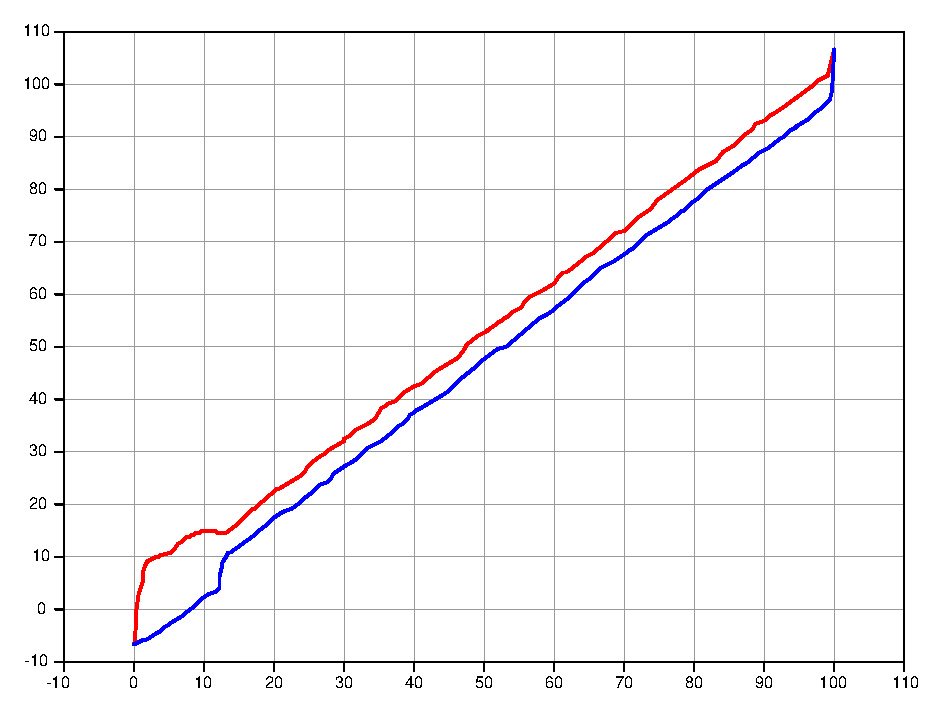
\includegraphics[width=15.5cm]{i01424x01.eps}$$

Hva er diagnosen din av denne ventilsignaturen? Hvilke fysiske problem(er) bør teknikeren begynne å lete etter ved inspeksjon av ventilen?

\vskip 20pt \vbox{\hrule \hbox{\strut \vrule{} {\bf Forslag til sokratisk diskusjon} \vrule} \hrule}

\begin{itemize}
\item{} En nyttig problemløsningsmetode i situasjoner med graf er å la grafen ``fortelle deg'' hva som skjer trinn for trinn over tid når du følger den fra den ene ytterenden til den andre. Prøv dette: Start i nedre venstre hjørne og følg det øvre (røde) sporet steg for steg som om du spiller av ventilåpningen over tid, og tolk grafen i form av spindelposisjon og aktuatortrykk (påført kraft). Beskriv hva grafen ``forteller'' deg når du følger den fra den ene enden til den andre.
\end{itemize}

\underbar{file i01424}
%(END_QUESTION)





%(BEGIN_ANSWER)

Denne ventilen opplever tydelig mer friksjon når pluggen nærmer seg setet. Hvis dette er en cage-guided globeventil, vil jeg foreslå å se etter mekanisk interferens mellom stempel og bur som følge av feilinnretting av delene eller dårlig maskinering. En annen mulighet er friksjon mellom spindel og pakning i samme (nesten lukket til lukket) posisjon.
 
%(END_ANSWER)





%(BEGIN_NOTES)


%INDEX% Final Control Elements, valve: diagnostic signature for pneumatic actuator

%(END_NOTES)

